\documentclass[10pt,twocolumn]{article}
\usepackage{graphicx} % Required for inserting images
\usepackage{oxy-comp}
\usepackage[style=numeric]{biblatex}
\bibliography{references}

\pdfinfo{
    /Title (Creating a multi-media batch-mint pipeline for NFT)
    /Author (Victor Zhu)
}

\title{Creating a multi-media batch-mint pipeline for NFT}
\author{Victor Zhu}
\affiliation{Occidental College}
\email{hzhu@oxy.edu}





\begin{document}

\maketitle
\abstract
The rise of Non-Fungible Tokens (NFTs) has ushered in a transformative era for digital assets, providing artists, creators, and collectors with new avenues to monetize and showcase their creative work. This academic paper comprehensively explores my project on developing a batch-mint NFTs pipeline. Our investigation delves into the diverse functionalities of this pipeline, its societal impact, potential applications, and the ethical considerations it entails. Moreover, we delve into the crucial role of NFTs and smart contracts in reshaping the dynamics of digital ownership and exchange dynamics. By interweaving theoretical insights with practical considerations, our research offers a holistic understanding of the broader implications of this project and its potential to foster growth and opportunities within the vibrant NFT ecosystem.


\section{Introduction}
Non-Fungible Tokens (NFTs) have become a groundbreaking innovation in digital assets. Revolutionizing how artists, creators, and collectors monetize and showcase their work. This section provides a comprehensive overview of NFTs and smart contracts. It highlights their definition, characteristics, relation to blockchain technology, impact on the art and entertainment industries, and relation to my project.

An NFT is "a digital asset that can come in the form of art, music, in-game items, videos, and more. They are bought and sold online, frequently with cryptocurrency, and they are generally encoded with the same underlying software as many cryptos."\cite{forbesdefination} Unlike traditional cryptocurrencies like Bitcoin, NFTs are distinct and cannot be exchanged one-to-one. Each NFT possesses unique properties and attributes that make it one-of-a-kind, such as its scarcity, rarity, demand, and authenticity. NFTs are non-fungible, meaning each token holds its distinct value and cannot be replicated or interchanged with another token. This uniqueness enables artists and creators to attach intellectual property rights, provenance, and authenticity to their digital creations, enhancing their value and exclusivity.

NFTs are stored on blockchain technology, a decentralized and transparent digital ledger. The NFTs eco-system "relies on blockchain for accounting their content and transactions to ensure user integrity, privacy, and reputation".\cite{blockchainmeta} By leveraging blockchain, NFTs guarantee transparency and authenticity, assuring buyers of their digital assets' verifiable ownership and provenance.

The advent of NFTs has opened up many opportunities for artists, creators, and collectors to monetize and showcase their work in previously inconceivable ways. With NFTs, artists can directly sell their digital creations, granting them control over the distribution and sale of their work. Furthermore, NFTs enable creators to receive royalties for subsequent sales of their digital assets, ensuring a sustainable revenue stream that extends beyond the initial sale.

Notable case studies have demonstrated the immense impact of NFTs on the art and entertainment industries. One example is the sale of digital artwork by the artist Beeple for a staggering  69 million. This historic sale not only showcased the commercial value of digital art but also solidified the position of NFTs as a legitimate and viable medium for artistic expression. \cite{nftmoney}

The influence of NFTs extends well beyond the realm of traditional art and has also penetrated deeply into the entertainment industry. In decentralized virtual worlds such as Decentraland, plots of virtual real estate have been sold as NFTs, with transaction prices reaching millions of dollars. These transactions underscore the escalating demand for immersive digital experiences and collectors' readiness to invest in virtual assets.

The capacity for artists, creators, and collectors to capitalize on their digital creations has allowed NFTs to redefine the conventional art market, prompting a significant paradigm shift in how value is ascribed to digital assets. The assurance of transparency and security, made possible through blockchain technology, has fostered trust and confidence among buyers and collectors. This has facilitated the development of a vibrant ecosystem for digital art and collectibles.

In conclusion, NFTs signify a transformative force within the landscape of digital assets, empowering artists, creators, and collectors to monetize and exhibit their work in ways previously unimaginable. The unique characteristics of NFTs, their reliance on blockchain technology, and the noteworthy instances of NFT transactions all contribute to the paradigm shift observed within the art and entertainment sectors. As the NFT ecosystem continues to mature and evolve, it is anticipated to present novel opportunities and challenges, further revolutionizing the creative landscape for artists and creators alike.

My project is about creating a pipeline for minting multiple NFTs simultaneously. Usually, NFT markets like Opensea do not have a function allowing you to mint multiple NFTs simultaneously. Many artists have many similar NFTs they want to upload at once. Without my project, they will have to mint the NFTs with different contracts each time. It is very inconvenient for artists who want to mint 10, 50, or even 100 NFTs simultaneously.  However, there are other options. Such as minting NFTs with multiple cpu; however, while manually utilizing multiple CPUs to mint items in parallel is possible, it often requires more effort, coordination, financial support, and monitoring compared to batch minting with code. By leveraging code, you can achieve higher efficiency, scalability, consistency, error handling, and automation, making the minting process more streamlined and manageable. Another option would be using one of many third-party websites that will mint the NFTs for you, such as thirdweb and others. Yet, these websites will need a serious effort to check if they can be trusted. From a security perspective, these sites may lack necessary protective measures against cyber attacks, leaving personal information, including private keys, vulnerable to theft. Users may also fall prey to phishing attacks, leading to the inadvertent disclosure of sensitive information on counterfeit platforms. Financially, these unsafe sites may need to be clearer about the true costs of minting NFTs, such as gas fees and commissions, resulting in unanticipated financial obligations. There's also a risk of encountering fraudulent schemes, where websites vanish post-payment, leaving creators needing their NFTs and funds. My pipeline is much safer and more personal than the online ones.  All the user needs is to enter the user information, then deploy the smart contract I provided and run the script main.py. There is no hidden fee, hidden transaction, no Malware. It will never leave or steal from you. My project will keep your NFTs safe and sound.  
\section{Technical Background}
For the execution of this project, several programming languages were employed, including JavaScript, Python, and Solidity. While it is anticipated that most readers are familiar with JavaScript and Python, a brief explanation will be provided for a comprehensive understanding. JavaScript is primarily used for enhancing interactivity within web pages. At the same time, Python, due to its readability and wide range of applications, is utilized across various domains, from web development to data analysis. Solidity, a statically-typed programming language designed for developing smart contracts on the Ethereum Blockchain, is also pivotal in this project.

In the execution of this project, JavaScript was employed for uploading the Non-Fungible Tokens (NFTs) to the InterPlanetary File System (IPFS). To enhance the user experience by simplifying interactions with these JavaScript files, a Python script was developed. Lastly, Solidity, an object-oriented programming language for writing smart contracts, was utilized to write the ERC-1155 smart contract. Following, a comprehensive explanation of the IPFS system and smart contracts will be provided to ensure a complete understanding of these key project components. 

A crucial component of this project is the InterPlanetary File System (IPFS), an innovative peer-to-peer network for storing and sharing data in a distributed file system.  IPFS is a "decentralized system because it loads the content from thousands of peers instead of one centralized server. Every piece of data is cryptographically hashed, resulting in a safe, unique content identifier: CID." IPFS is a vital tool in the world of NFTs. It helps keep the digital assets that are tied to the tokens always accessible and authentic. IPFS is conceptually a decentralized storage system where your files are stored across multiple locations, not just in one place. This makes it incredibly hard for the files ever to disappear or get modified, ensuring the value of your NFT stays intact. When a file is added to IPFS, it gets a unique cryptographic hash(CID). This hash acts like an ID card for the file and also serves as proof that the file hasn't been tampered with, so the owner will be alert if the files are changed.

smart contracts, at their core, are "simply programs stored on a blockchain that run when predetermined conditions are met. They typically are used to automate the execution of an agreement so that all participants can be immediately certain of the outcome without any intermediary’s involvement or time loss. They can also automate a workflow, triggering the next action when conditions are met."\cite{IBMSmartcontractt} They are foundational for decentralized applications (dApps) and autonomous organizations (DAOs). Smart contracts are instrumental to Non-Fungible Tokens (NFTs), particularly to the ERC-721 and ERC-1155 standards on the Ethereum blockchain. The ERC-721 standard pioneered the definition of NFTs, fostering the creation and trade of unique, indivisible tokens. Each ERC-721 token is distinctive, with each token ID tied to a unique asset, paving the way for digital scarcity.

The ERC-1155 standard, introduced by Enjin, is a multi-token standard for the Ethereum blockchain that allows for the creation and management of both fungible and non-fungible tokens within a single, smart contract. This standard was proposed by Witek Radomski and published as an Ethereum Improvement Proposal (EIP) under the number EIP-1155. This standard notably benefits gaming platforms and applications where various asset types are transacted.\cite{erc115standered}

One of the key advantages of ERC-1155 is its ability to optimize the use of blockchain resources. With ERC-20 and ERC-721, each token required a separate smart contract, leading to increased gas costs and network congestion. In contrast, ERC-1155 allows multiple tokens to be managed within a single contract, reducing the overall gas fees and enhancing scalability. ERC-1155 supports both fungible tokens (representing identical units of value) and non-fungible tokens (representing unique assets). This versatility makes it suitable for various use cases, particularly in the gaming industry. Game developers can utilize ERC-1155 to create in-game items, currencies, and collectibles, allowing for seamless integration, efficient management, and enhanced user experiences.\cite{erc115standered}

The significance of ERC-1155 extends beyond gaming. It enables the creation of diverse asset classes within a unified framework, facilitating tokenization across multiple domains, such as digital art, real-world assets, and decentralized finance (DeFi) protocols. This standard also supports advanced functionalities like batch transfers, which can significantly reduce transaction costs and improve user interactions.
\section{Prior Work}
The implementation of ERC-1155 in the project is a strategic choice for its ability to mint multiple non-fungible tokens (NFTs) simultaneously. The selection of this standard over others, such as ERC-721, stems from its more efficient approach to token management.

Distinctly, ERC-721 generates individual smart contracts for each NFT, while ERC-1155 stores all token types within a single smart contract. This arrangement not only simplifies token management but also makes the process more economical. The unique efficiency of ERC-1155 lies in its ability to create and manage both fungible and non-fungible tokens in a unified manner, offering considerable flexibility and versatility.\cite{ERC-721_vs_ERC-1155}

Within the ERC-1155 contract, each token is given a unique token ID, representing either a fungible or a non-fungible asset. This property has been leveraged in the project to ensure the uniqueness of each NFT minted. The token ID is a differentiating identifier, making each NFT distinct from the rest.

In minting multiple NFTs simultaneously, the project harnesses the power of the batch minting function inherent in the ERC-1155 standard. This function bestows upon the contract owner or authorized users the ability to specify the token ID, the quantity of each NFT to be minted, and any additional attributes or metadata associated with the tokens. This feature streamlines the minting process and optimizes the allocation of resources.\cite{erc115standered}

Contrarily, projects such as “How to: batch minting your NFTs” presented by Liarco DevTips, chose to use the ERC-721 standard. The choice of ERC-721 for batch minting revolves around the granularity and customization it provides for each NFT during the minting process. The advantage of this approach lies in the ability to individually specify unique attributes, properties, or metadata for each NFT.

However, batch minting using ERC-721 carries the drawback of higher gas costs compared to ERC-1155. With each token requiring a separate transaction and deployment of a distinct smart contract, the costs pile up, resulting in higher transaction fees. The multitude of individual transactions also has the potential to slow down processing times.\cite{ERC-721_stand}

To summarize, the decision to utilize ERC-1155 in the project is anchored in its intrinsic efficiencies and flexible capabilities. These capabilities extend to the consolidation of all tokens under a single contract, the creation and management of both fungible and non-fungible tokens, and the ability to mint multiple unique NFTs simultaneously. While ERC-721 allows for greater individual customization, its higher gas costs and potential for slower processing times make it a less optimal choice for this specific project.

The judicious selection of smart contract standards, in this case, ERC-1155, contributes significantly to the project's success. It underscores the importance of aligning the choice of technology with the project's objectives and operational requirements. By prioritizing efficiency, flexibility, and cost-effectiveness, the project ensures a smooth and economic minting process, enhancing the overall user experience and performance of the batch minting pipeline.



\section{Method}
The javascript for most of my script because it is the industry standard. Moreover, thanks to its powerful toolset, JavaScript is a prime choice for minting NFTs on Ethereum. Two JavaScript libraries, web3.js, and ethers.js, come to the forefront in the Ethereum ecosystem. They equip developers with various functions, simplifying interactions with the blockchain. These include dealing with smart contracts, transactions, and token standards like ERC-721 and ERC-1155 for NFTs and ERC-20 for other tokens. 

In minting NFTs, a critical step involves interacting with Ethereum smart contracts. JavaScript and the libraries mentioned make it easier for developers to create, sign, and send transactions to smart contracts, making the whole process seamless.

Moreover, the Ethereum environment frequently employs JavaScript Object Notation (JSON). JSON is an accessible, machine-readable format that neatly encapsulates data. In Ethereum, it's often used to present smart contract interfaces and transaction data. Given that JSON is part of the JavaScript language, working with such data structures in Ethereum becomes considerably more straightforward.

In essence, JavaScript's broad functionality, combined with Ethereum-focused tools and native support for JSON, make it a compelling choice for projects that involve minting NFTs. Its use enables developers to navigate the complexities of blockchain technology with greater ease.  

 Python is used  to call all the javascript scripts for no other reason than a personal reference 

This project was embarked upon with the ERC-1155 standard being chosen over ERC-721. The primary motivation for this selection was driven by the fact that the project did not demand the elaborate functionalities offered by ERC-721. Instead, a swift and straightforward solution was sought, and ERC-1155 emerged as a front runner due to its efficiency and reduced gas costs.

ERC-1155 enables the minting of multiple NFTs under a single contract, which streamlines the minting process and obviates the need for distinct smart contracts for each token. For projects constrained by the amount of cryptocurrency available, a contract that substantially lowers gas costs and bolsters overall efficiency becomes a highly desirable option. The simplicity and convenience proffered by ERC-1155 make it a fitting choice for such projects, facilitating seamless and cost-effective batch minting of NFTs.\cite{ERC-721_vs_ERC-1155}

At the onset of this undertaking, a series of misconceptions surfaced. There was a belief that the creation of IPFS addresses would enable NFTs to automatically mint themselves. In order to automate the file transfer process and encode the files into Base64 format, unnecessary functionality was introduced to both image.js and metadata.js. In a somewhat misguided endeavor, an attempt was even made to document everything into a CSV file and run a for loop to read from the CSV files in a smart contract via Remix IDE. However, these initiatives met with considerable roadblocks. The previously functional code turned into a perplexing enigma, despite numerous hours invested in debugging and problem-solving. Eventually, the conclusion was drawn that the additional functionality was superfluous, leading to the decision to revert to the original codebase.

Through this process, the component that recorded the IPFS addresses into a CSV file with each run was identified as being useful. Despite this minor victory, a significant challenge remained, which was the minting of NFTs via a contract. It required a vital decision concerning the choice of smart contract. Following careful consideration, ERC 1155 was selected.

However, ERC 1155 did not come without its drawbacks. It permitted the minting of multiple tokens, but under a single IPFS address, which fell short of the project's envisioned outcome. A system where each token could be minted with a unique IPFS address was desired. Unfortunately, deploying ERC 1155 via Remix did not offer a solution for minting with multiple IPFS addresses, necessitating a search for alternatives.

An attempt was made to use Hardhat to deploy the contract outside of Remix with the aim of writing a loop to append different IPFS addresses, but this endeavor proved unsuccessful. The decision was made to revert to Remix for the deployment of the contract. Subsequently, a JavaScript script titled 'minting' was crafted, which made it possible to mint NFTs with multiple unique IPFS addresses using the contract obtained from Remix.
\section{Evaluation Metrics}

At the inception of this project, a strategic plan was used to create a pipeline capable of minting numerous non-fungible tokens (NFTs) simultaneously with diverse media. The project aimed to minimize user input and maximize output, providing a seamless and efficient user experience.

To measure the project's success in achieving this objective,  three different evaluation criterion was established: ease of use, the volume of concurrent NFT minting, and versatility in handling various media forms.

“Ease of use” are defined, in the context of my paper, by several key elements: Accessibility, Simplicity, Efficient Workflow, Customization and Flexibility, and Sufficient Documentation and Support. Each component acts as a cog in the machine that collectively contributes to the project's user-friendliness and practical functionality.

The accessibility was aimed to be easily understood and navigable. Clear visual cues, logical flow, and simplified user interactions were incorporated to reduce users' cognitive load, allowing them to carry out tasks seamlessly and efficiently without needing substantial prior system knowledge.

Simplicity, ensuring users could quickly grasp the system's functionality and use it effectively. By reducing the time and effort required to learn, we hoped to increase overall productivity and ease of use.

The project emphasized an Efficient Workflow, a systematic and organized process for users to execute their tasks within the system. By streamlining processes and reducing extraneous steps, the workflow fosters productivity and minimizes the potential for errors.

In terms of Customization and Flexibility, the system was designed to cater to individual user needs and preferences. It allows users to modify settings, interface elements, and workflows to suit their specific requirements, leading to enhanced user satisfaction and productivity.

Sufficient Documentation and Support was another key component. Comprehensive guides, FAQs, tutorials, and customer support were provided to help users understand, troubleshoot, and optimize their system use. This provision bolsters user confidence and ensures a smoother and more successful interaction with the system.

By adhering to these standards, the project was aimed at providing a user-friendly and enjoyable experience. A successful and rewarding user experience increases the likelihood of project adoption, thereby fulfilling the project's initial goal - an efficient, versatile, and user-friendly pipeline for batch-minting NFTs.
\section{Result and Discussion}

\subsection {Accessibility}
In the execution of this project, the code developed necessitates running a specific script to perform its intended function. However, a current limitation is that all files can only be executed within an Integrated Development Environment (IDE). This implies that, while the code is well-documented with comments, there remains a necessity for explicit instructions within the code to guide users in understanding their expected actions.
However, to address this, a comprehensive Readme has been prepared and is available on the GitHub page. This Readme is designed to assist users in navigating the code and understanding how to use it effectively.
Despite these measures, when evaluating against the first standard of 'ease of use'—an Intuitive User Interface—self-assessment renders a score of 5 out of 10.

In the current stage of the project, there remains potential for enhancing the intuitive nature of the user interface, to better meet this established standard. Future development will focus on improving this score by refining user interface design and providing clearer in-code instructions for users.

\subsection{Simplicity}
Evaluating the project against the standard of Simplicity reveals a largely positive outcome. Once the initial setup is complete—processes that need only be executed once—the users need only place their chosen files in the 'export' directory and run 'main.py'. While there may be some initial challenges in mastering these steps, users can quickly become adept at navigating the system. Consequently, a score of 9 out of 10 has been assigned for this metric.

\subsection{Efficient Workflow}

Upon assessing the system based on the standard of an Efficient Workflow, the results are somewhat mixed. On the one hand, the pipeline design, in its core, requires only the execution of a single script - 'main.py', to run the entirety of the project. This streamlined approach encourages efficiency and simplicity.

However, it is noteworthy that several critical setup tasks necessitate completion prior to the execution of the main script. These tasks encompass finding an API key from the Moralis web application, uploading the files to the user's web folder with the IPFS address, deciding upon the network for minting NFTs, finding the private key from the user's wallet, and compiling and deploying the provided contract on the Remix platform to acquire the abi and contract address. Following these steps, users are required to place the files intended for minting into the 'export' folder.

After the successful completion of these preliminary tasks, users can then run 'main.py' to initiate the minting process for all files placed in the 'export' folder. While these setup tasks, excluding the action of placing files into the 'export' folder, only need to be executed once, they are essential for the correct minting of NFTs. Consequently, these steps are unable to be further simplified. For the Efficient Workflow standard, a score of 6 out of 10 is assigned.

The standard for Efficient Workflow denotes a systematic and organized procedure enabling users to perform their tasks within the system. This standard strives to streamline processes and minimize unnecessary steps, thereby promoting productivity and reducing potential errors. Within this context, while the single script execution design is a positive attribute, there is room for improvement in simplifying and streamlining the setup tasks for increased efficiency and ease of use.

\subsection{Can it be Customized and have Flexibility?}

When considered in the context of the standard of Customization and Flexibility, the project code exhibits a degree of adaptability, although it does contain some limitations. 

Users can modify certain aspects of the code by inputting their own API key, private key, contract address, and network URL, which enables customization to fit individual requirements. However, beyond these adjustable elements, further customization options are limited and may not be necessary given the specific nature of the project's functions.

In terms of flexibility, the current project's code exhibits some rigidity. Attempts to alter certain parts of the code were met with non-functional outcomes, suggesting limited malleability. Therefore, in relation to the Customization and Flexibility standard, the project receives a score of 7 out of 10.

The standard of Customization and Flexibility reflects the extent to which a system can be personalized to meet specific user needs and preferences, and how readily it can adapt to changes. An ideal system allows users to modify settings, interface elements, and workflows to suit their unique requirements, improving user satisfaction and productivity. Moreover, it can adjust and function efficiently in response to modifications. While the project achieves partial success in meeting these expectations, there is room for improvement in terms of enhancing the code's flexibility.

\subsection{Does it have Documentation and Support}
When analyzed against the Sufficient Documentation and Support standard, the project reveals strengths and improvement areas. The code is meticulously commented, elucidating various sections' and functions' purpose and functionality. This facilitates user understanding and navigation. Furthermore, a comprehensive Readme file is available on the GitHub repository, providing valuable instructions and insights on system use.
However, providing ongoing support for users is not currently planned, and this could impact user experience. Particularly in complex or unanticipated situations, users may require assistance to troubleshoot issues or optimize system utilization. The absence of such support could potentially hinder efficient system interaction and result in a less satisfactory user experience. 
From this perspective, while the project successfully incorporates well-commented code and a detailed Readme, the lack of ongoing support services is a limitation. Future considerations may include strategies for providing user support, whether through collaborative platforms, automated assistance, or community-driven resources, to enhance the project's alignment with this standard. Consequently, a 6 out of 10 scores is assigned when considering the Sufficient Documentation and Support standard.

\subsection{For how many NFTs mint at once?}
Regarding the number of NFTs that can be minted simultaneously, the system has demonstrated effective functionality with up to 50 NFTs. However, the system's design and capabilities extend beyond this figure, with the potential for minting significantly larger batches of NFTs in a single operation.

The experiment of minting ten NFTs was constrained not by the system's capacity but rather by the limited availability of Matics. Therefore, this test served as a proof of concept and should not be seen as the system's upper limit. Indeed, the architecture is geared towards enabling larger-scale operations, efficiently managing multiple NFT minting processes simultaneously. 

Thus, while the current testing environment allowed for the successful minting of 50 NFTs in a single operation, it should be recognized that the system is robustly equipped for more extensive minting tasks, depending on the availability of the necessary resources such as Matics.

\subsection{Will it take different media as NFTs?} 
When examining the capability of the system to process various media types as Non-Fungible Tokens (NFTs), the response is twofold. On one hand, the system is designed to accept a wide range of media files for transformation into NFTs, illustrating its broad applicability and versatility.

However, a current system limitation lies in its ability to handle diverse file formats. While it can process numerous media types, it currently converts all input files into the .png image format. This constraint is due to the specifications of the upload folder utilized, which exclusively accepts image files. Consequently, even though different media types are initially accepted, the final minted NFTs are presented in a uniform .png format.

It is essential to acknowledge that this characteristic does not devalue the diversity of the original content. Nonetheless, it is worth noting that potential future developments could aim to maintain the original media formats, thereby further enhancing the flexibility and capacity of the system to create NFTs from various media types. 

\section{Ethical Considerations}
When assessing the ethical ramifications of the batch minting of NFTs, it is crucial to examine several primary areas of concern carefully:
Environmental Considerations: The process of batch-minting NFTs entails executing a significant volume of transactions on the blockchain network. This activity necessitates substantial computational power and energy, contributing to the blockchain's environmental impact. This is especially true when the network is based on energy-intensive consensus mechanisms such as proof-of-work. The ethical dimension surfaces when considering the carbon emissions and the environmental footprint connected to high-volume minting operations.

\subsection{Scarcity and Exclusivity} 
NFTs traditionally embody a sense of exclusivity and uniqueness. Mass minting of NFTs could risk diluting the individual exclusivity of each item and potentially devaluing the broader NFT ecosystem. Such a scenario raises concerns among artists, creators, and collectors who are keen to preserve the unique value and scarcity of their NFTs.

\subsection{Quality Assurance and Originality}
 The automated nature of batch minting may pose questions around the quality and originality of the NFTs being generated. If not adequately curated or supervised, automated processes could yield low-quality or derivative content that infringes upon copyright or intellectual property rights. This possibility may threaten the authenticity and trustworthiness typically associated with NFTs.

\subsection{Representation and Bias}
The ethical implications of batch minting are not solely technological but also social. The potential influence on diversity and representation within the NFT space is a vital concern. If the batch minting process does not consciously ensure diversity in creators, artists, or content, it could perpetuate existing disparities and imbalances within the digital and art realms. Ethical practices necessitate the elimination of potential biases and a commitment to equitable representation in the minting process.

\subsection{Energy Consumption}
Previously, every time someone made a transaction on the Ethereum network, which included buying or selling an NFT, 128 kilograms of carbon dioxide were generated. This is the same amount of energy the average home consumes over two weeks.\cite{nftrisk} However, in September 2022, the Ethereum blockchain implemented a new consensus mechanism called "proof of stake," resulting in a significant reduction of over 99 percent in Ethereum's energy consumption. The consensus mechanism is responsible for securing the blockchain was previously based on "proof of work," which was largely responsible for the substantial energy emissions associated with Ethereum.

These ethical considerations warrant a comprehensive evaluation of the broader impact and implications of batch-minting NFTs. This includes reducing environmental impacts, preserving the integrity and value of NFTs, fostering diversity, and ensuring equitable distribution of resources and opportunities. By undertaking rigorous research, adhering to ethical principles, and embracing diverse viewpoints, developers and stakeholders can strive toward an equitable and responsible approach to batch minting.

\section{Future Work and Conclusion}
My project is about one of the newest technologies: NFTs. As written above, the core characteristic of NFTs is decentralized and its uniqueness. This is both a curse and a blessing. The decentralization of NFTs is a blessing because there is no censorship. Every artist could own their tool of production and distribution.  However, decentralization also means no regulation  for selling and buying parties. This put them at risk of fraud and other harm. The uniqueness defines the value of the NFTs, but since there is no regulation, anybody could just plagiarise the artists’ products. These factors and combined with the recent crash of the crypto market, made the NFTs market goes down in value dramatically.
However, I do believe the NFTs market will rise again after the AI technology surge and 3D printing technology. AI technology makes creating art easy than ever before. The NFTs market was still a niche market. However, as AI technology improves, people can create movies, murals even television series. Selling them as NFT will give them more autonomy other than relying on big businesses. With more advanced 3D printing technology, people can actually feel their NFTs. This will add more value to the NFTs. The seller could also sell schematics of things such as cars, beds, or even houses. With advanced 3D printing technology, they are able to build from the NFTs schematics.

There are still many parts of this project that can be improved. The project would be simpler if I could deploy my contract with hardhat. It will cut short the processing time and also lose a few steps. If I could deploy the contract with hardhat, I do not need to use remix to deploy it. I do not need to find the abi and contract address on Remix. Rather I could do it all by command line. I think I will work on that in the future.
\section{Timineline}
2022 May 31 to August 4 Building a classifier for all the NFTs that I want to upload

2022 December 15 Start to build the pipeline

2023 January 24 Coding to create  metadata.js and images.js for uploading NFT in NFT.

2023 February 24 Continue to add more functionality to the javascript, metadata.js, and images.js

2023 March 13 Adding python script to run the javascript

2023 April 5 Adandon new  metadata.js and images.js. Re-code the old one.

2023 April 10 Finish the new  metadata.js and images.js

2023 April 20 Add in javascript code to mint NFTs in the IDE, and another javascript for hardhat

2023 April 30 Abandon hard hat and use Remix instead



\section{Code Document}
\begin{figure}[tb]
  \centering
  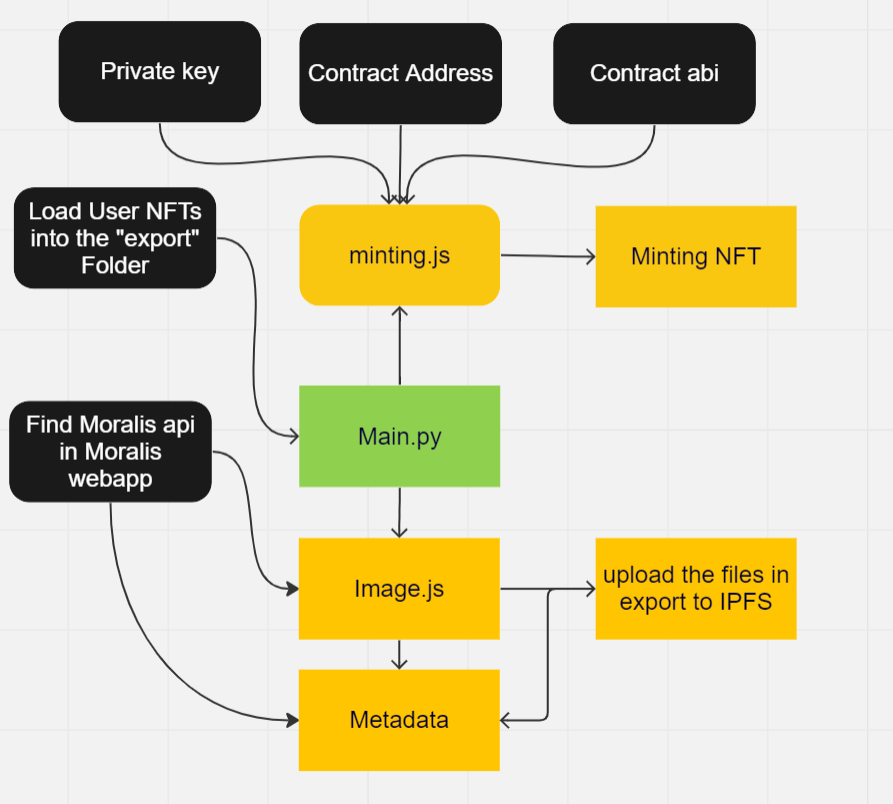
\includegraphics[width=0.5\textwidth]{flowchart.png}
  \caption{Flowchart of my code.}
  \label{fig:1}
\end{figure}






\printbibliography

\end{document}

